% *********************************************************************
% © 2021-2022 Jeremy Sylvestre
%
% Permission is granted to copy, distribute and/or modify this document
% under the terms of the GNU Free Documentation License, Version 1.3 or
% any later version published by the Free Software Foundation; with no
% Invariant Sections, no Front-Cover Texts, and no Back-Cover Texts. A
% copy of the license is included in the appendix entitled “GNU Free
% Documentation License” that appears in the output document of this
% PreTeXt source code. All trademarks™ are the registered® marks of
% their respective owners.
%
% *********************************************************************

\newcommand*{\xmin}{1.25}
\newcommand*{\xmax}{4.75}
\newcommand*{\ymin}{-2}
\newcommand*{\ymax}{5.5}
\newcommand*{\func}{\x * \x * \x * \x / 4 - 3 * \x * \x * \x + 23 * \x * \x / 2 - 14 * \x + 3}

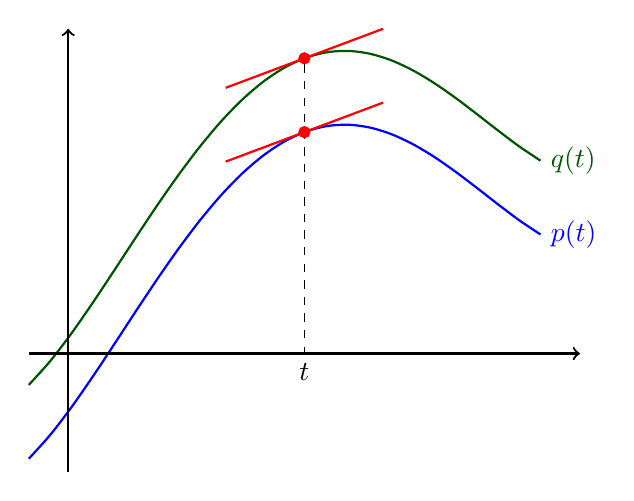
\begin{tikzpicture}
[
	closedpt/.style={circle,draw,fill,inner sep=0pt,minimum size=4pt},
	openpt/.style={circle,draw,inner sep=0pt,minimum size=4pt},
	xscale=2,
	yscale=0.75
]

	\begin{scope}[yshift=1.25cm]

		% shifted graph
		\draw[thick, green!33!black, domain=1.25:4.5, smooth] plot (\x,{\func}) node[right] {$q(t)$};

		\draw[thick,red] (2.5,3.25) -- (3.5,4.25);
		\node[closedpt,red] at (3,3.75) (qcentre) {};

	\end{scope}

	\draw[dashed] (qcentre) -- (3,0) node[below] {$t$};

	% example graph
	\draw[thick, blue, domain=1.25:4.5, smooth] plot (\x,{\func}) node[right] {$p(t)$};

	\draw[thick,red] (2.5,3.25) -- (3.5,4.25);
	\node[closedpt,red] at (3,3.75) (qcentre) {};

	% axes
	\draw[->,thick] (\xmin,0) -- (\xmax,0);% node[below left] {$t$};
	\draw[->,thick] (1.5,\ymin) -- (1.5,\ymax);



\end{tikzpicture}
